% $Header: /cvsroot/latex-beamer/latex-beamer/solutions/generic-talks/generic-ornate-15min-45min.en.tex,v 1.4 2004/10/07 20:53:08 tantau Exp $

\documentclass{beamer}

% This file is a solution template for:

% - Giving a talk on some subject.
% - The talk is between 15min and 45min long.
% - Style is ornate.

% Copyright 2004 by Till Tantau <tantau@users.sourceforge.net>.
%
% In principle, this file can be redistributed and/or modified under
% the terms of the GNU Public License, version 2.
%
% However, this file is supposed to be a template to be modified
% for your own needs. For this reason, if you use this file as a
% template and not specifically distribute it as part of a another
% package/program, I grant the extra permission to freely copy and
% modify this file as you see fit and even to delete this copyright
% notice. 
% Modified 7 June 2006 by B.K. Muite

\mode<presentation>
{
  \usetheme{Singapore}
  % or ...

  \setbeamercovered{transparent}
  % or whatever (possibly just delete it)
}

\usepackage[english]{babel}
% or whatever

\usepackage[latin1]{inputenc}
%\usepackage{multimedia}
\usepackage{amsmath,amsthm}
\usepackage{amssymb}
\usepackage{epstopdf}
\usepackage{times,bm}
\usepackage{subfigure,url}
\usepackage{algpseudocode}
\usepackage{algorithm}
\usepackage{hyperref}
%\usepackage{textcomp}
\usepackage{graphicx}
\usepackage{setspace}
\usepackage{listings}
\lstset{showstringspaces=false,showtabs=false,tabsize=2,captionpos=b,}
\providecommand{\ssub}[2]{#1_{\scriptscriptstyle #2}}
%\usepackage[T1]{fontenc}
% Or whatever. Note that the encoding and the font should match. If T1
% does not look nice, try deleting the line with the fontenc.
%\logo{\includegraphics[height=0.8cm]{./Figures/TartuLogo2.png}\vspace{1pt}}
\title[]
{Some computational tools for the humanities}

\author[]{Benson Muite}

\institute[]{\url{benson.muite@ut.ee}\\
                  \url{http://kodu.ut.ee/~benson/}                  }
\date[]{10 June 2016}

\begin{document}

\begin{frame}
  \titlepage
\end{frame}

% Since this a solution template for a generic talk, very little can
% be said about how it should be structured. However, the talk length
% of between 15min and 45min and the theme suggest that you stick to
% the following rules:  

% - Exactly two or three sections (other than the summary).
% - At *most* three subsections per section.
% - Talk about 30s to 2min per frame. So there should be between about
%   15 and 30 frames, all told.

\begin{frame}
\frametitle{Some Links}
\begin{itemize}
\item  \url{https://github.com/Digitaalhumanitaaria/Digitaalhumanitaaria.github.io/blob/master/storage/seminarpreparation.md}
\item  \url{http://digitaalhumanitaaria.github.io/storage/seminarpreparation}
\end{itemize}
\end{frame}


\begin{frame}
\frametitle{Outline}
\begin{itemize}
\item Git
\item LaTeX
\item Pandoc
\item Parallel R
\item Language Evolution Simulation
\end{itemize}
\end{frame}

\begin{frame}
\frametitle{Git}
\begin{figure}[t]
\centering
   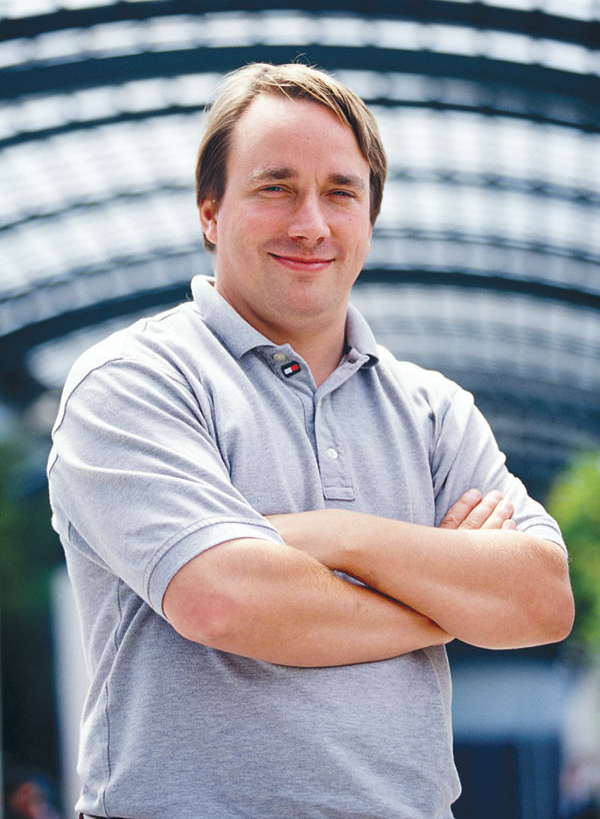
\includegraphics[scale = 0.3]{Linus_Torvalds.png}
\caption{Linus Torvalds, created of Git and Linux, Linux grand tsar.}
\end{figure}
\end{frame}

\begin{frame}
\frametitle{Git}
\begin{itemize}
\item Distributed version control
\item Allow multiple people to work on a project together
\item Keep a history of additions to the project
\item Works best for text files where compression and tracking algorithms are effective, though can also use it to store other files
\end{itemize}
\end{frame}

\begin{frame}
\frametitle{Git providers}
\begin{itemize}
\item Github \url{https://github.com/}
\item Bitbucket \url{https://bitbucket.org/}
\item Gitlab \url{https://about.gitlab.com/}
\item You?
\end{itemize}
\end{frame}

\begin{frame}
\frametitle{TeX}
\begin{figure}[t]
  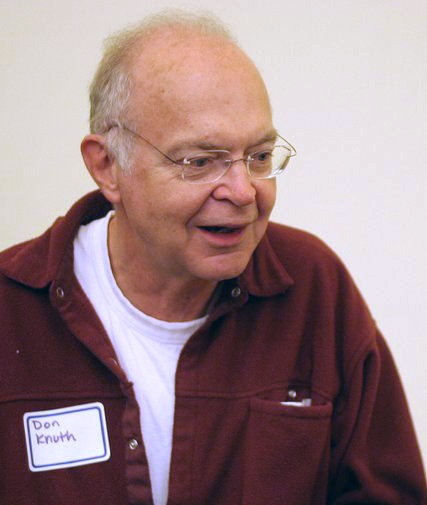
\includegraphics[scale = 0.3]{Donald_Knuth.png}
\caption{Donald Knuth created TeX.}
\end{figure}
\end{frame}

\begin{frame}
\frametitle{TeX}
\begin{figure}[t]
   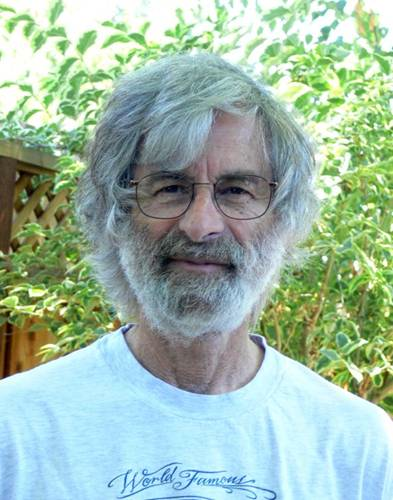
\includegraphics[scale = 0.3]{Leslie_Lamport.png}
\caption{Leslie Lamport created LaTeX.}
\end{figure}
\end{frame}

\begin{frame}
\frametitle{LaTeX}
\begin{itemize}
\item Want better support in other languages
\item Being open can incorporate this -- but need to develop a community
\item Since a markup language, can try to use extra contextual information when processing files
\item One area to start with is bibliographies -- biblatex package \url{https://github.com/Digitaalhumanitaaria/biblatex}
\end{itemize}
\end{frame}

\begin{frame}
\frametitle{Pandoc}
\begin{itemize}
\item Many different markup languages
\item Want to be able to translate from one markup language to another
\item In many cases, equivalent types of commands, eg. title, subtitle, bold formatting etc
\item Pandoc is an attempt to do this
\item Still needs some human cleanup
\end{itemize}
\end{frame}

\begin{frame}
\frametitle{Parallel R}
\begin{itemize}
\item Programming with Big Data in R (pbdR) \url{http://r-pbd.org/}
\begin{itemize}
\item[i)] open source project to allow you to do statistical analysis on large data sets
\item[ii)] can be useful for processing large data corpora
\item[iii)] PCA (principle component analysis) example
\end{itemize}
\item \url{https://github.com/vijayachitrabio/biohpc}
\end{itemize}
\end{frame}

\begin{frame}
\frametitle{Example from social sciences}
\begin{itemize}
\item Abrams-Strogatz model for language death
\item \begin{align*} 
&{} \frac{\mathrm{d}x}{\mathrm{d}t}=yp_{yx}-xp_{xy}\\
&{} p_{yx}=csx^a \quad p_{xy}=c(1-s)(1-x)^a\\
&{} y=1-x
\end{align*}
\item $x$ fraction of population speakers of  language $x$, $y$ fraction of population speakers of  language $x$, $p_{xy}$ probability of switching from language $x$ to $y$, $p_{yx}$ probability of switching from language $y$ to $x$, $c$ time scaling constant, $a$ influence of population size on probability of switching language (claim $a\approx1.3$ for many groups), $s$ - relative status of language 
\end{itemize}
\end{frame}

\begin{frame}
\frametitle{Example from social sciences}
\begin{itemize}
\item Patriarca-Heinsalu model 
\item \begin{align*}
&{} N1_t &=& k(s1 N1^a N2 - s2 N2^a N1) + N1_{xx}+N1_{yy} \\
&{} & &+ \alpha N1 - \alpha N1 (N1+N2)/KK
\\&{} N2_t &=& k(s2 N2^a N1 - s1 N1^a N2) + N2_{xx}+N2_{yy} \\
&{}   & &  + \alpha N2 - \alpha N2 (N1+N2)/KK
\end{align*} 
\item $N_i$ population of speakers of language $i$,  $k$ rate coefficient, $a$ model fitting parameter, $s_i$ relative status, $\alpha$ Malthus growth rate, $KK$ carrying capacity
\end{itemize}
\end{frame}

\begin{frame}
\frametitle{Conclusions and further work}
\begin{itemize}
\item Many of these tools work best on command line
\item This takes time to learn how to use
\item Advantage is automation for often repeated procedures which are slow to repeat yourself in a GUI
\item Also allows customization and generation of workflows suited to you
\item Get an account on an HPC cluster try some of these tools
\item Provide some interesting data sets and we can help you use these tools
\end{itemize}
\end{frame}

\begin{frame}
\frametitle{References}
\begin{itemize}
 \item Abrams, D.M. and Strogatz, S.H. ``Modelling the dynamics of language death'' Nature \textbf{424}, 900 (2013) \url{http://dx.doi.org/10.1088/1367-2630/13/3/033007}
\item Appelbaum, J. ``Donald Knuth'' \url{https://en.wikipedia.org/wiki/Donald\_Knuth\#/media/File:KnuthAtOpenContentAlliance.jpg}
\item Lamport, L. ``Leslie Lamport" \url{https://en.wikipedia.org/wiki/Leslie\_Lamport\#/media/File:Leslie\_Lamport.jpg} 
\end{itemize}
\end{frame}

\begin{frame}
\frametitle{References}
\begin{itemize}
\item Linux Magazine ``Linus Torvalds'' \url{https://en.wikipedia.org/wiki/Linus\_Torvalds\#/media/File:Linus\_Torvalds.jpeg} 
\item Patriarca, M. and Heinsalu, E. ``Influence of geography on language competition'' Physica A: Statistical Mechanics and its Applications
\textbf{388}(2--3), 174-186, (2009) \url{http://dx.doi.org/doi:10.1016/j.physa.2008.09.034} \url{http://arxiv.org/abs/0807.3100v2}
\end{itemize}
\end{frame}

\begin{frame}
\frametitle{Acknowledgements}
{\footnotesize
\begin{itemize}
\item Oleg Batra\u{s}ev
\item Els Heinsalu
\item Artjom Lind
\item Anders Martoja
\item \begin{minipage}{1.0\linewidth}
\begin{center}
\begin{tabular}{ccc}
  
\includegraphics[height=0.950cm]{./EUrdf.png} &
  
\includegraphics[height=0.950cm]{./EstoniaFlag.png} &
  \includegraphics[height=0.950cm]{./excs.png} 
\end{tabular}
\end{center}
\end{minipage}
\end{itemize}
}
\end{frame}


\end{document}
